
% $Id$

\documentclass[11pt,a4paper]{article}
\usepackage{graphicx}
\usepackage[english]{babel}
\usepackage[latin1]{inputenc}
\usepackage{amssymb}
\usepackage{isabelle,isabellesym,pdfsetup}

\isabellestyle{it}
\renewcommand{\isamarkupsubsubsection}[1]{\subsubsection*{#1}}
\newcommand{\isasymRrightarrow}{\isamath{\Rrightarrow}}

\begin{document}

\title{Fundamental Properties of Lambda-calculus}
\author{Tobias Nipkow \\ Stefan Berghofer}
\maketitle

\tableofcontents

\begin{center}
  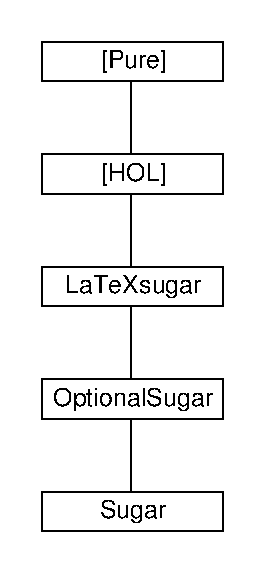
\includegraphics[scale=0.7]{session_graph}  
\end{center}

\newpage

\parindent 0pt \parskip 0.5ex

\input{Lambda}
\input{Commutation}
\input{ParRed}
\input{Eta}
\input{ListApplication}
\input{ListOrder}
\input{ListBeta}
\input{InductTermi}
\input{Type}

\end{document}
